% --------------------------------------------------------------------

\chapter[Variable Objects]{Variable Objects}
\def\chpname{variables}\label{chp:\chpname}

Chapter editors:
\credit{AshishMahabal},
\credit{lmwalkowicz}.

% \noindent {\it
% Mike Lund, Ashish Mahabal, Stephen Ridgway,
% Lucianne Walkowicz, Rahul Biswas, Michelle Lochner,
% Jeonghee Rho, Eric Bellm...
% }

% --------------------------------------------------------------------


\section{Introduction}

Variable objects are defined as those that exhibit brightness changes, either periodic or non-periodic, which are detected in quiescence and non-destructive to the object itself. Variable objects span a wide range in timescale-of-interest (sometimes even within a single class of objects), and so different science cases benefit from different sampling strategies. These strategies may be significantly disparate from one another, sometimes even mutually exclusive; competing objectives described in this chapter and the next are therefore at the heart of LSST observing strategy and cadence design.

Below we develop a number of key science cases for LSST studies of variable objects, associating them with related metrics that can be used within the Metrics Analysis Framework (MAF) to understand the impact of a given survey strategy realization on the scientific results for that case. The science cases outlined are by no means exhaustive, but rather are motivated by providing key quantitative examples of LSST's performance given any particular deployment of survey strategy. The authors encourage community contribution of similar cases, where the scientific outcome can be quantified using specific metrics.



%When evaluating a particular observation or series of observations in
%light of how they perform for a specific science case, it may be
%helpful to think of metrics as lying along a continuum between
%discovery and characterization. Discovery requires a minimum amount of
%information to recognize an event or object as a candidate of
%interest, which necessarily involves some level of bare-bones
%characterization (upon which said recognition is based); rich
%characterization, on the other hand, implies that an event may not
%only be recognized as a candidate of interest, but basic properties of
%the event or object may be determined from the observation (e.g.
%including but not limited to classification of the event). The
%interpretation of a given metric along this continuum has implications
%for the subsequent action and analysis required, particularly as
%regards possible follow-up observations with other facilities.

%Target types are here grouped in subsections by variability
%characteristics, but as will be seen, this does not mean that all
%targets in a group require a common cadence, since the times scales
%may vary dramatically.  Acquiring suitable data for a wide range of
%time scales presents a fundamental problem for LSST, since the
%available $~$800 visits to a field over the survey cannot be deployed
%so as to usefully sample all time scales at all times.  This fact
%leads to the concept of a non-uniform survey, in which parts of the
%sky are visited more frequently part of the time.  The merits of such
%options must be traded against the benefits of a more uniform survey
%strategy.

\begin{center}
\begin{tabular}{| l | p{8cm} |l | l |}
\hline Periodic Variable Type & Examples of target science & Amplitude & Timescale\\
\hline
RR Lyrae & Galactic structure, distance ladder, RR Lyrae properties&  large &  day \\
Cepheids & Distance ladder, cepheid properties&  large &  day \\
Long Period Variables & Distance ladder, LPV properties & large  &  weeks \\
Short period pulsators & Instability strip, white dwarf interior properties, evolution&  small & min  \\
Periodic binaries & Eclipses, physical properties of stars, distances, ages, evolution, apsidal precession, mass transfer induced period changes, Applegate effect &  small &  hr-day \\
Rotational Modulation & Gyrochronology, stellar activity& small  &  days \\
Young stellar populations & Star and planet formation, accretion physics & small  &  min-days \\
 \hline \end{tabular}
 \end{center}
 
 \section{The Cepheid Mass-Luminosity Relation}

Classical Cepheids begin to pulsate once the evolve up the giant branch and execute blueward loops on the HR diagram that take them 
into the Instability Strip. Cepheid masses and luminosities in the instability strip are connected through the Mass-Luminosity (ML) relation.
This ML relation is strongly dependent on stellar evolution physics. Canonical/Non-canonical ML
relations arise from varying treatments of convective core overshoot and mass loss (Brocato and Castellani 1992, Bono et al 2000,
Marconi et al 2013).

Stellar pulsation models adopt a given ML relation and then compute a theoretical light curve for a range of
different temperatures and metallicities. This theoretical light curve can then be transformed into LSST wavebands using
stellar atmospheres (B20 and references therein) and quantitatively compared to observed LSST light curves through Fourier decomposition of the
form
$$V = A_0 + \sum_{k=1}^{k=N}(A_k cos(k\omega t) + {\phi}_k),$$
where $\omega = 2\pi/P,$ with $P$ the period, $N$ is the order of the fit. The coefficients $R_{k1}=A_k/A_1$ and 
${\phi}_{k1}={\phi}_k - k{\phi}_1$ can be computed for both theoretical and LSST observed light curves. These coefficients
are sensitive to the adopted $ML$ relation and other global parameters such as metallicity and effective temperature.
By utilizing such a decomposition,
the multiwavelength light curves that the LSST will produce for both Cepheids and RR Lyraes can rigorously constrain Cepheid and RR
Lyrae global stellar parameters such as the ML relation. Of course, knowledge of the ML relation through this approach can then
lead to another "theoretical" distance scale using both Cepheids and RR Lyraes. 
However, in the case of Cepheids, given good enough cadence in LSST bands and thus an accurate Fourier decomposition with precisely known
Fourier parameters, it will be possible to discriminate between canonical and non-canonical ML relations and thus provide constraints
for stellar evolution physics.

Bhardwaj et al (2014) describes in detail the way the quantitative structure of Cepheid and RR Lyrae light curves vary with
period and optical band. Given appropriate cadence, LSST light curves will provide accurate Fourier decompositions at multiple 
wavelengths that can significantly augment these results and provide an important database with which to connect quantitative
aspects of Cepheid and RR Lyrae light curve structure to pulsation envelope physics. Two examples are the following.
\begin{itemize}
\item{1)} RRab stars found in stripe 82 of the
SDSS exhibit a flat PC relation at minimum light at certain SDSS colors but not at others. LSST observations of RRab stars will be able
to augment this result and investigate if there are any links to the structural properties of observed light curves.
\item{2)} Short period ($\log P \le 0.4$) FU Cepheids in the SMC exhibit a noticeable break in their $(V-I)$ PC relation at certain phases of pulsation
phases. At the same period, the Fourier parameter $R_{21}$ displays a strong turnover. LSST data will be important in seeing if this result extends 
to LSST colors.
\end{itemize}

Bhardwaj et al (2014 and references therein, Bhardwaj et al 2015) have clearly demonstrated how Cepheid and RR Lyrae
Period-Color(PC)/Period-Luminosity (PL)/
Period-Wesenheit(PW)/Period-Luminosity-Color(PLC) relations vary significantly both as a function pulsation phase and period and observation band. 
The LSST database on Cepheids and RR Lyraes will provide an excelletn database tofurther investigate the variation of these relations with pulsation phase
with a view to understanding pulsation physics and constraining theoeretical models. Currently, the literatiure only
discusses these relations at mean light, that is the average over pulsation phase. Yet this averaging process clearly masks some
dependencies: there are pulsation phases with very high/low PL/PC dispersion and there are some phases where the relation is highly nonlinear.
In the era of precision cosmology, it is important to understand the tools that we use to construct a distance scale. The LSST database on
Cepheids and RR Lyraes will be an important database with which to investigate the multipahse properties of PL/PC/PW/PLC relations.

What cadence is required for "accurate multiwavelength Fourier decomposition"? 
Probably more opsim experiments are required but one way forward is to consider a cadence and then simulate observed light curves with this 
cadence, Fourier analyze these light curves with errors on Fourier parameters (Petersen 1980) and the compare with a preliminary grid
of theoretical model light curves.



\subsection{Description of Relevant Metrics}
\label{sec:keyword:variablemetrics}

Despite the range in scientific motivation for the cases presented below, there are some common metrics that are widely applicable (or may be combined in a variety of ways with other metrics to suit a variety of applications).

%\subsection{Metrics}
%\label{sec:keyword:metrics}

\begin{center}
\begin{tabular}{| p{5cm} |p{10cm} |}
\hline Metric & Description\\
\hline
Eclipsing/transiting system discovery & Fraction of discoveries vs fractional duration of eclipse\\
Lightcurve shape recovery & ... \\
%Transiting exoplanets (depth dependent) & Fraction of discoveries vs fractional duration of eclipse\\
Phase gap & Histogram vs period of the median and maximum phase gaps achieved in all fields\\
Period determination (period dependent) & Fraction of targets vs survey duration, for which the period can be determined to 5-sigma confidence\\
Period variability (period dependent) & Fraction of targets vs survey duration, for which a period change of 1\% can be determined with 5-sigma confidence\\
  \hline \end{tabular}
 \end{center}

The ability to identify that an object is periodic, and to correctly determine that object's period, are widely applicable measures of discovery. In the case of regular variables (as outlined below), these two measures together can uniquely identify a population. Other kinds of periodic systems (transiting planets for example) also require a measurement of periodicity, but have a much wider range of relevant periods, and looser requirements on the strictness of that periodicity.

Lund et al. (2015; \url{http://arxiv.org/pdf/1508.03175.pdf}) discuss three metrics that have been incorporated into the MAF. Two of these metrics deal explicitly with time variable behavior: a) observational triplets, and b) detection of periodic variability.

%%%%%%%%%%%%%%%%%%%%%%%%%%%%%%%%%
\begin{figure}[tbh!]
%\vskip -4.1in
%\hskip -0.5in
%\includegraphics[angle=0,width=1.19\hsize:,clip]{figs/enigma1189_earlySNe.pdf}
%\vskip -4.0in
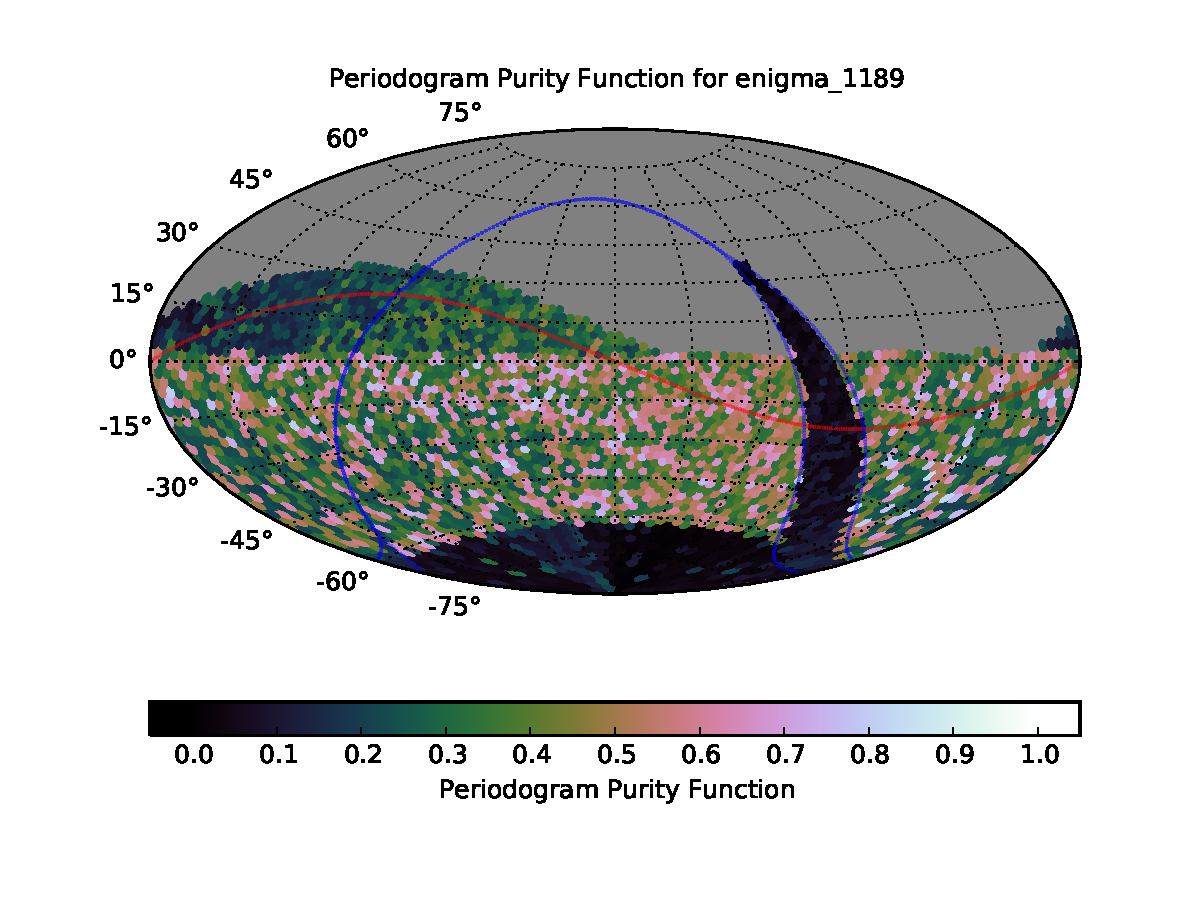
\includegraphics{figs/variables/enigma_1189_PeriodogramPurity_OPSI_SkyMap.pdf}
\caption{The value for the Periodogram Purity Function for candidate Baseline Cadence \opsimdbref{db:enigma}.
The Periodogram Purity Function provides a measure of the power lost due to aliasing.}
\label{fig:enigmaPeriodogramPurity}
\end{figure}
%%%%%%%%%%%%%%%%%%%%%%%%%%%%%%%%%


%%%%%%%%%%%%%%%%%%%%%%%%%%%%%%%%%
\begin{figure}[tbh!]
%\vskip -4.1in
%\hskip -0.5in
%\includegraphics[angle=0,width=1.19\hsize:,clip]{figs/enigma1189_earlySNe.pdf}
%\vskip -4.0in
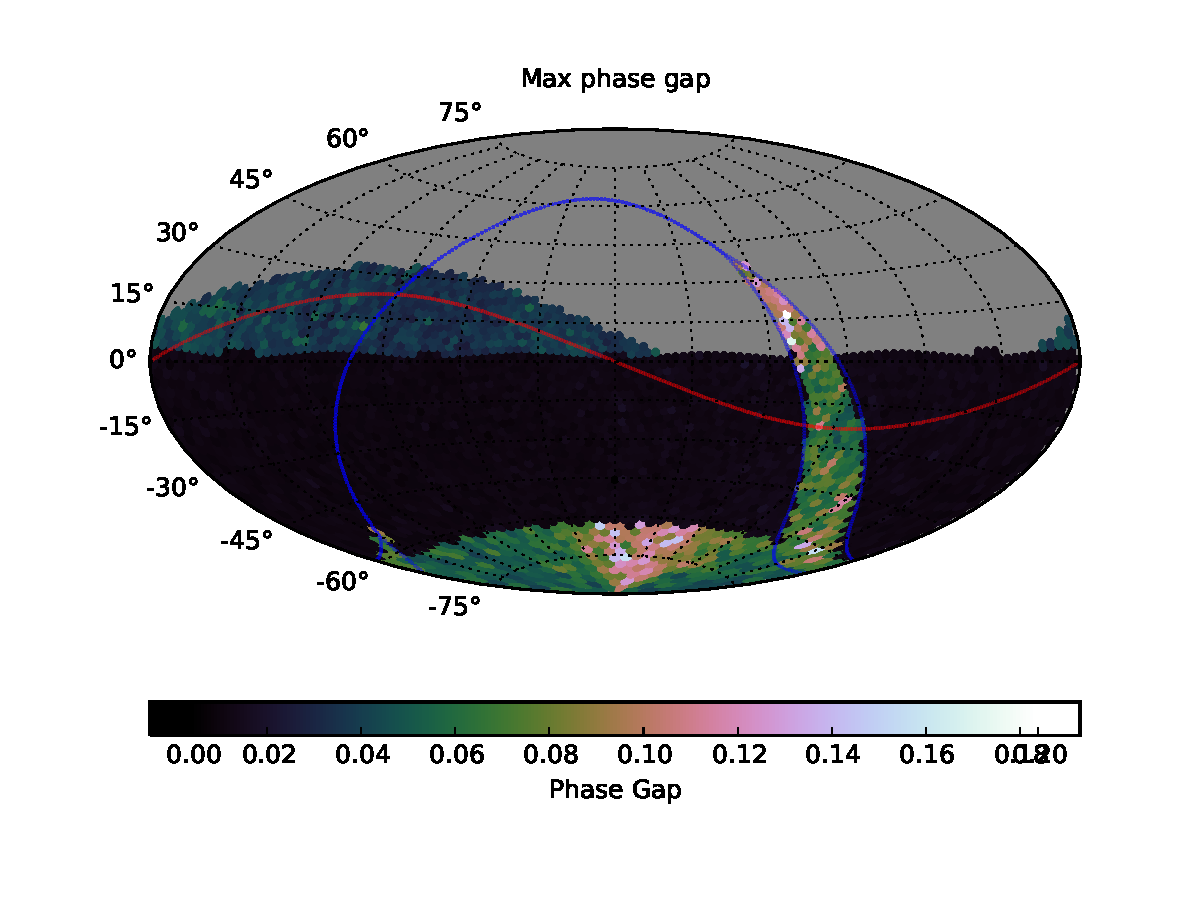
\includegraphics{figs/variables/enigma_1189_Phase_Gap_MedianGap_OPSI_SkyMap.pdf}
\caption{The median phase gap for candidate Baseline Cadence \opsimdbref{db:enigma}.
The PhaseGapMetric looks at periods between 3 and 35 days by default.}
\label{fig:enigmaMedianGap}
\end{figure}
%%%%%%%%%%%%%%%%%%%%%%%%%%%%%%%%%

%%%%%%%%%%%%%%%%%%%%%%%%%%%%%%%%%
\begin{figure}[tbh!]
%\vskip -4.1in
%\hskip -0.5in
%\includegraphics[angle=0,width=1.19\hsize:,clip]{figs/enigma1189_earlySNe.pdf}
%\vskip -4.0in
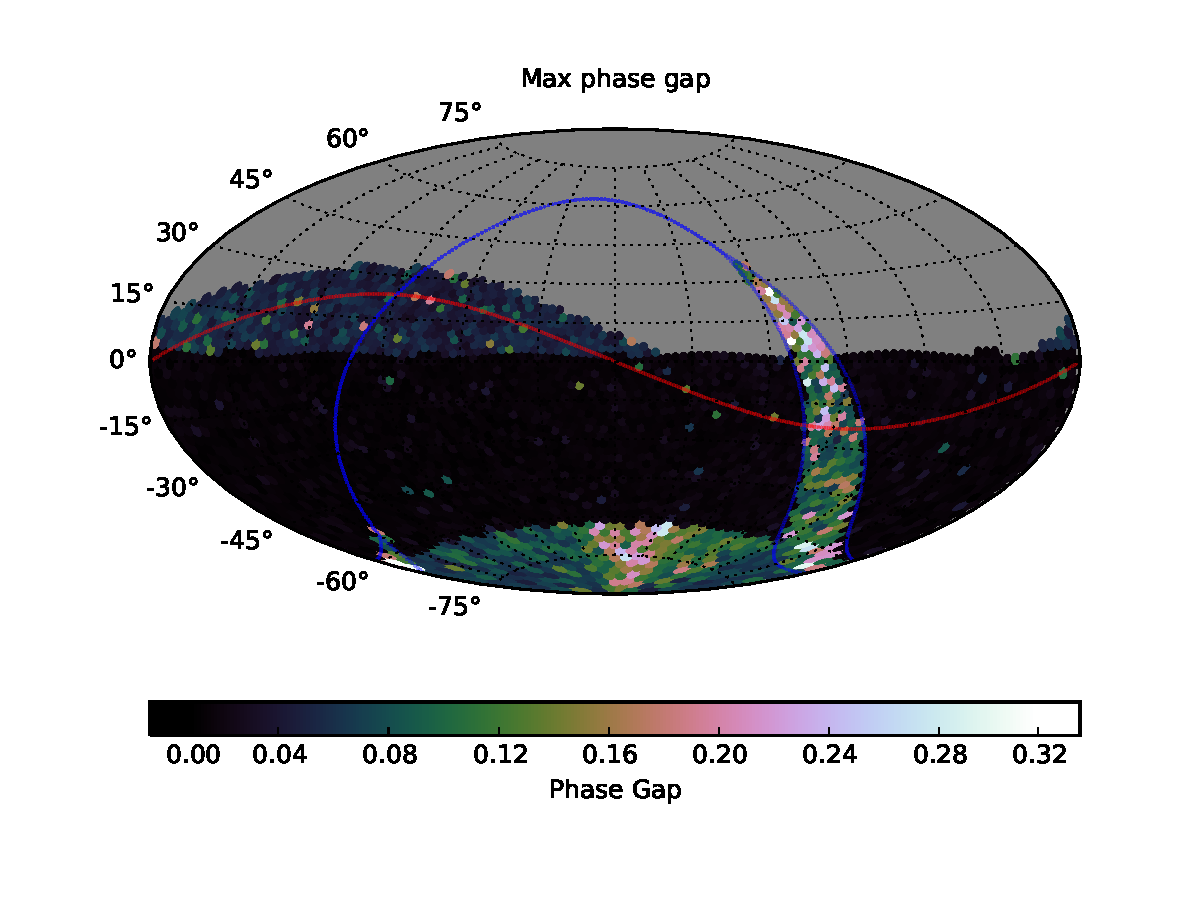
\includegraphics{figs/variables/enigma_1189_Phase_Gap_LargestGap_OPSI_SkyMap.pdf}
\caption{The maximum phase gap for candidate Baseline Cadence \opsimdbref{db:enigma}.
The PhaseGapMetric looks at periods between 3 and 35 days by default.}
\label{fig:enigmaMaxGap}
\end{figure}
%%%%%%%%%%%%%%%%%%%%%%%%%%%%%%%%%

\subsubsection{Periodogram purity function (PeriodicMetric)}
This metric calculates the Fourier power spectral window function of each field (Roberts et al. 1987) as a means of quantifying the completeness of phase coverage for a given periodic variable. The periodogram purity is defined as 1 minus the Fourier power spectral window function. in the perfect case, all power in the window function is concentrated in a delta function at zero, and is zero at all other frequencies. As power ``leaks'' away from the correct frequency as a consequence of discrete, non-ideal data sampling, the periodogram becomes more structured. For the purposes of MAF metrics, which are designed to quantify performance as a single number, the periodogram purity is quantified as the minimum value of the periodogram purity function at non-zero frequency shifts; the ideal case would be a periodogram purity metric value of 1.

\subsubsection{Phase Gap Metric (PhaseGapMetric)}

The Phase Gap Metric is designed to examine the largest phase gaps in the observing schedule. For a given point in the sky, a series of periods are randomly selected (by default, 5 periods), with a default minimum of 3 days and maximum of 35 days. The largest phase gap for each period is calculated, and the metric plots the median (\autoref{fig:enigmaMediangap}) and maximum (\autoref{fig:enigmaMediangap}) of this subset of values that contains the maximum phase gap per period. The Phase Gap Metric is part of varMetrics.

\subsubsection{Period Deviation Metric (PeriodDeviationMetric)}

The Period Deviation Metric calculates the error in recovering the correct period of sinusoid using a given observing schedule and a Lomb-Scargle periodogram. For a given point in the sky, a series of periods are randomly selected (by default, 5 periods), and the metric returns the worst period deviation, and the period at which this occurred. The Period Deviation Metric is part of varMetrics.

%\subsection{Proposed Metrics}

%The following is a raw list of metric ideas; these need specificity and further description.

%FWHM of the window function (to quantify sampling)

%Maximum hour angle difference

%Fraction of discoveries vs fractional duration of eclipse

%Fraction of targets vs survey duration, for which the period can be determined to 5-sigma confidence

%Fraction of targets vs survey duration, for which a period change of 1$\%$ can be determined with 5-sigma confidence




% --------------------------------------------------------------------


% ====================================================================
%+
% NAME:
%    section-name.tex
%
% ELEVATOR PITCH:
%    Explain in a few sentences what the relevant discovery or
%    measurement is going to be discussed, and what will be important
%    about it. This is for the browsing reader to get a quick feel
%    for what this section is about.
%
% COMMENTS:
%
%
% BUGS:
%
%
% AUTHORS:
%    Phil Marshall (@drphilmarshall)  - put your name and GitHub username here!
%-
% ====================================================================

\section{Discovery of Periodic Pulsating Variables}
\def\secname{periodicvariables}\label{sec:\secname}

\noindent{\it Lucianne M. Walkowicz, Stephen Ridgway, \&c} % (Writing team)

% This individual section will need to describe the particular
% discoveries and measurements that are being targeted in this section's
% science case. It will be helpful to think of a ``science case" as a
% ``science project" that the authors {\it actually plan to do}. Then,
% the sections can follow the tried and tested format of an observing
% proposal: a brief description of the investigation, with references,
% followed by a technical feasibility piece. This latter part will need
% to be quantified using the MAF framework, via a set of metrics that
% need to be computed for any given observing strategy to quantify its
% impact on the described science case. Ideally, these metrics would be
% combined in a well-motivated figure of merit. The section can conclude
% with a discussion of any risks that have been identified, and how
% these could be mitigated.

Regular variables, such as Cepheids and RR Lyraes, are valuable tracers of Galactic structure and cosmic distance. In this case of these and other strictly (or nearly-strictly) periodic variables, data from different cycles of observation can be phase-folded to create a more fully sampled lightcurve as LSST visits will occur effectively at random phases. In a 10-year survey, most periodic stars of almost any period will benefit from excellent phase coverage in all filters (only a very small period range close to the sidereal day will be poorly observed). Therefore, most implementations of the LSST observing strategy will provide good sampling of periodic variables.

However, different implementations of the survey may result in different resulting sample sizes of these periodic variables, and may also affect the environments in which these stars are discovered. In this section, we create a framework for understanding how current implementations of the observing strategy influence (or even bias) the resultant sample size and environments where these important tracers may be identified. 

\subsection{Tracing Galactic Structure with RR Lyrae}

Oluseyi et al. 2012 [INSERT REF] carried out an extensive simulation of period and lightcurve shape recovery of RR Lyrae variables using an early OpSim run \textit{opsim1_29}. Correctly identifying the period aids in building the sample of interest, whereas fitting the lightcurve shape makes it possible to measure the metallicity of the star. In their simulation, they employed both a Fourier analysis and template matching to recover the lightcurve shape, finding that template matching yielded a more accurate lightcurve shape measurement in the presence of sparse data. 

The results of this simulation showed that the vast majority of RR Lyrae will be discovered by the baseline observing strategy (as deployed in \textit{opsim1_29}) within 5 years of survey operations. Half of both RRLab and RRLc stars will be found out to $\sim$600 kpc and $\sim$250 kpc (respectively) by the end of the 10-year main survey, and template matching techniques for lightcurve shape recovery will provide metallicities to $\sim$0.15dex. This incredible sample will enable discovery of Galactic tidal stream and neighboring dwarf galaxies throughout much of the Local Group (Ivezic,Z., Tyson, J. A., Allsman, R., et al. 2008a, arXiv: 0805.2366) 

% --------------------------------------------------------------------

\subsection{The Cepheid Cosmic Distance Ladder}

Classical cepheids remain an essential step in the cosmic distance ladder. Their calibration is based largely on LMC cepheids and known (assumed) distance of the LMC.  The associated errors, while uncertain, are believed to be of $\>\sim$7\%. (Madore, Barry F.; Freedman, Wendy L. (2009). "Concerning the Slope of the Cepheid Period?Luminosity Relation". The Astrophysical Journal 696 (2): 1498. arXiv:0902.3747. Bibcode:2009ApJ...696.1498M. doi:10.1088/0004-637X/696/2/1498.) New developments in galactic studies are poised to support substantially improved descriptive information concerning nearby galactic cepheids, with possible substantial reductions in this error, by accurately securing the PL slope and zero point.

Cepheid calibration errors are associated in part with uncertainties in extinction, both interstellar and in some cases circumstellar, and in metalicity.  At present, the direct, local calibration of cepheids is limited by the availability of a few direct distance measurements, obtained with HST, with errors $\sim$10\%.  The GAIA mission is expected to return $\sim$9000 Galactic cepheids, of all periods, colors and metallicities, with distance errors less than 10\% (many of them much less) - Windmark, F.; Lindegren, L.; Hobbs, D., 2011A&A...530A..76W. It is expected to deliver at least 1000 cepheids in the LMC with expected mean distance error $\sim$7-8\% (Clementini (2010) - 011EAS....45..267C).  GAIA, as well as other methods, will also support determination of the 3-d map of galactic interstellar extinction - including possible variations in the extinction law. These rich data sets will be supported with direct measurements of cepheid diameters (A. Merand et al, A\&A in press) and advances in stellar hydrodynamics (E. Mundprecht et al, 2013MNRAS.435.3191M) which will provide theoretical and empirical basis for calibrations to reconcile known physics with observational correction factors.

Galactic cepheids will generally be too bright for LSST, but cepheids in the local group are sufficiently bright that LSST photometry will be limited by calibration errors rather than by brightness.  This dataset will provide superb support for integration of GAIA-based galactic cepheid studies with extra-galactic cepheid studies.

GAIA will provide similar precision data with the potential to identify or support distance determinations from many other galactic star types.  LSST photometric catalogs will represent a uniquely extensive and complete database for such investigations.

% --------------------------------------------------------------------

\subsection{OpSim Analysis}
\label{sec:keyword:analysis}


Several metrics currently exist in the MAF for evaluating how LSST survey strategy affect the recovery of periodic sources. 

The periodogram purity function (PeriodicMetric, which effectively quantifies aliasing introduced into periodogram analysis from the sampling of the lightcurve)

and period deviation metric (PeriodDeviationMetric) all return relevant information 

phase gap metric (PhaseGapMetric),

the evaluate the periodicity of the source lightcurve and its coverage in phase space (the latter being relevant for shape recovery). 

Recreating the template matching results of the Oluseyi et al. (2012) simulation requires sampling specific input lightcurves and comparing with the library of available shapes; this necessarily requires a step outside of the MAF, but can easily be enabled using the lightcurve simulation tool [NAME OF FED'S LIGHTCURVE TOOL].
 



Current simulations of the main survey show a broad uniformity of visits, with thorough randomization of visit phase per period, giving very good phase coverage with minimum phase gaps.


% --------------------------------------------------------------------

\subsection{Discussion}
\label{sec:keyword:discussion}

For periodic variable science, two cadence characteristics should be avoided:
\begin{itemize}
\item an exactly uniform spacing of visits (which is anyway virtually impossible); \
\item a very non-uniform distribution, such as most visits concentrated in a few survey years.
 \end{itemize}

A metric for maximum phase gap will guard against the possibility that a very unusual cadence might compromise the random sampling of periodic variables.

In each case, it would help to jump-start science programs if some fraction of targets had more complete measurements early in the survey.


% ====================================================================

\navigationbar


% --------------------------------------------------------------------

% ====================================================================
%+
% NAME:
%    planets.tex
%
% CHAPTER:
%    variables.tex
%
% ELEVATOR PITCH:
%-
% ====================================================================

% \section{Probing Planet Populations with LSST}
\subsection{Probing Planet Populations with LSST}
\def\secname{planets}\label{sec:\secname}

\credit{lundmb},
\credit{shporer},
\credit{stassun}

This section describes the unique discovery space for
extrasolar planets with LSST, namely,
planets in relatively unexplored environments.

% \subsubsection{Planets In Relatively Unexplored Environments}

A large number of exoplanets have been discovered over the past few
decades, with over 1500 exoplanets now confirmed. These discoveries are
primarily the result of two detection methods: The radial velocity (RV)
method where the planet's minimum mass is measured, and the transit
method where the planet radius is measured and RV follow-up allows the
measurement of the planet's mass and hence mean density. Other methods
are currently being developed and use to discover an increasing number of
planets, including the microlensing method and direct imaging. In
addition, the Gaia mission is expected to discover a large number of
planets using astrometry \citep{2014exha.book.....P}.

The {\it Kepler} mission has an additional almost 4000 planet
candidates. While these planet candidates have not been confirmed, the
sample is significant enough that planet characteristics can be studied
statistically, including radius and period distributions and planet
occurrence rates. LSST will extend previous transiting planet searches
by observing stellar populations that have generally not been
well-studied by previous transiting planet searches, including star
clusters, the galactic bulge, red dwarfs, white dwarfs (see below), and
the Magellanic Clouds (see \autoref{sec:MCs:MC_exoplanets}). Most known
exoplanets have been found relatively nearby, as exoplanet systems with
measured distances have a median distance of around 80~pc, and 80\% of these
systems are within 320~pc (exoplanets.org). LSST is able to recover transiting
exoplanets at much larger distances, including in the galactic bulge and the
Large Magellanic Cloud, allowing for measurements of planet occurrence rates in
these other stellar environments
\citep{2015AJ....149...16L,2015AJ....150...34J}.
Red dwarfs have often been
underrepresented in searches that have focused on solar-mass stars, however red
dwarfs are plentiful, and better than 1 in 7 are expected to host earth-sized
planets in the habitable zone \citep{2015ApJ...807...45D}.

Another currently unexplored environment where LSST will be able to
probe the exoplanet population is planets orbiting white dwarfs (WDs).
Such systems teach us about the future evolution of planetary systems
with main-sequence primaries, including that of the Solar System. When a
WD is eclipsed by a planet (or any other faint low-mass object,
including a brown dwarf or a small star) the radius and temperature
ratios lead to a very deep eclipse, possibly a complete occultation,
where during eclipse the target can drop below the detection threshold.
The existence of planets orbiting WDs has been suggested
observationally
\citep[e.g.,][]{2009ApJ...694..805F,2009AJ....137.3191J,2010ApJ...722..725Z,2012ApJ...747..148D}.
and theoretically \citep[e.g.,][]{2010MNRAS.408..631N}.
A few brown dwarf companions were already discovered
\citep[e.g.,][]{2006Natur.442..543M,2012ApJ...759L..34C,2006Sci...314.1578L,2014MNRAS.445.2106L},
and \citet{2015Natur.526..546V}
recently discovered a disintegrating planetary body orbiting a WD
\citep[see also][]{2015arXiv151006434C,2016ApJ...818L...7G,2016MNRAS.458.3904R}.

While most of the sky that LSST will survey will be at much lower
cadences than transiting planet searches employ, a sufficient
understanding of the LSST efficiency for detecting planets combined with
the large number of targets may still provide significant results.
Additionally, the multiband nature of LSST provides an extra benefit, as
exoplanet transits are achromatic while many potential astrophysical
false positives, such as binary stars, are not.
Indeed, as demonstrated by \citet{2015AJ....149...16L}, the multi-band LSST light curves
can likely be combined to create merged light curves with denser sampling and effectively
higher cadence, enabling detection of transiting exoplanets. The deep-drilling fields in
particular should prove to be a rich trove of transiting exoplanet detections, with
transit-period recoverability rates as high as $\sim$50\% or more among Hot Jupiters around
solar-type stars out to distances of many kpc and even the Magellanic Clouds in some cases
\citep{2015AJ....149...16L,2015AJ....150...34J}.
Yields may be expected perhaps as early as the third year of LSST operations
(Jacklin et al., in prep).
The ability to detect transiting planets outside of the deep-drilling fields is less certain;
here the details of the cadence among the various passbands will likely be particularly
important to assess carefully.


\subsection{Metrics}
\label{sec:\secname:metrics}
The detection of transiting planets will be dependent on having observations
that will provide sufficient phase coverage for transiting planets, with periods
that can range from less than one day up to tens of days. In order to address
this range of periods, an initial metric that can be used to address the detection
of transiting planets is the Periodogram Purity Function, discussed more thoroughly
in Section~5.2.1.

\subsection{Discussion}
\label{sec:\secname:discussion}
In general, the detection of transiting exoplanets with LSST will rely on
a small subset of potentially detectable planets that can be sufficiently
separated from statistical noise, rather than a clear threshold in a planet's
properties that would distinguish detectable planets vs. nondetectable planets.
This will mean that the best calculation of planet yields will have to come
from simulations of light curves for large numbers of stellar systems in order
to characterize LSST. The computation time involved in this process is sufficiently
prohibitive to prevent a metric being developed based directly on these
simulated light curves, however future work may be able to map relationships
between metric values for individual fields and the corresponding numbers
of planets that can be detected.

%
% % --------------------------------------------------------------------
%
% \subsection{OpSim Analysis}
% \label{sec:\secname:analysis}
%
% % --------------------------------------------------------------------
%
% \subsection{Discussion}
% \label{sec:\secname:discussion}
%
% ====================================================================
%
% \subsection{Conclusions}
%
% Here we answer the ten questions posed in
% \autoref{sec:intro:evaluation:caseConclusions}:
%
% \begin{description}
%
% \item[Q1:] {\it Does the science case place any constraints on the
% tradeoff between the sky coverage and coadded depth? For example, should
% the sky coverage be maximized (to $\sim$30,000 deg$^2$, as e.g., in
% Pan-STARRS) or the number of detected galaxies (the current baseline but
% with 18,000 deg$^2$)?}
%
% \item[A1:] ...
%
% \item[Q2:] {\it Does the science case place any constraints on the
% tradeoff between uniformity of sampling and frequency of  sampling? For
% example, a rolling cadence can provide enhanced sample rates over a part
% of the survey or the entire survey for a designated time at the cost of
% reduced sample rate the rest of the time (while maintaining the nominal
% total visit counts).}
%
% \item[A2:] ...
%
% \item[Q3:] {\it Does the science case place any constraints on the
% tradeoff between the single-visit depth and the number of visits
% (especially in the $u$-band where longer exposures would minimize the
% impact of the readout noise)?}
%
% \item[A3:] ...
%
% \item[Q4:] {\it Does the science case place any constraints on the
% Galactic plane coverage (spatial coverage, temporal sampling, visits per
% band)?}
%
% \item[A4:] ...
%
% \item[Q5:] {\it Does the science case place any constraints on the
% fraction of observing time allocated to each band?}
%
% \item[A5:] ...
%
% \item[Q6:] {\it Does the science case place any constraints on the
% cadence for deep drilling fields?}
%
% \item[A6:] ...
%
% \item[Q7:] {\it Assuming two visits per night, would the science case
% benefit if they are obtained in the same band or not?}
%
% \item[A7:] ...
%
% \item[Q8:] {\it Will the case science benefit from a special cadence
% prescription during commissioning or early in the survey, such as:
% acquiring a full 10-year count of visits for a small area (either in all
% the bands or in a  selected set); a greatly enhanced cadence for a small
% area?}
%
% \item[A8:] ...
%
% \item[Q9:] {\it Does the science case place any constraints on the
% sampling of observing conditions (e.g., seeing, dark sky, airmass),
% possibly as a function of band, etc.?}
%
% \item[A9:] ...
%
% \item[Q10:] {\it Does the case have science drivers that would require
% real-time exposure time optimization to obtain nearly constant
% single-visit limiting depth?}
%
% \item[A10:] ...
%
% \end{description}
%
% ====================================================================

\navigationbar


% --------------------------------------------------------------------

% ====================================================================
%+
% NAME:
%    planets.tex
%
% CHAPTER:
%    variables.tex
%
% ELEVATOR PITCH:
%-
% ====================================================================

\section{Age-Mapping the Galaxy Using Gyrochronology}
\def\secname{rotatationalvariables}\label{sec:\secname}

This section describes recovering stellar rotation periods as a means to
mapping ages of stellar populations in the Galaxy.

\subsection{Recovery of Periods from Rotational Modulation}

% --------------------------------------------------------------------

\subsection{Metrics}
\label{sec:\secname:metrics}


% --------------------------------------------------------------------

\subsection{OpSim Analysis}
\label{sec:\secname:analysis}


% --------------------------------------------------------------------

\subsection{Discussion}
\label{sec:\secname:discussion}

% ====================================================================

\navigationbar


% --------------------------------------------------------------------


% ====================================================================
%+
% NAME:
%    section-name.tex
%
% ELEVATOR PITCH:
%    Explain in a few sentences what the relevant discovery or
%    measurement is going to be discussed, and what will be important
%    about it. This is for the browsing reader to get a quick feel
%    for what this section is about.
%
% COMMENTS:
%
%
% BUGS:
%
%
% AUTHORS:
%    Phil Marshall (@drphilmarshall)  - put your name and GitHub username here!
%-
% ====================================================================

\section{Discovery and Characterization of Young Stellar Populations}
\def\secname{periodicvariables}\label{sec:\secname}

\noindent{\it Author Name(s)} % (Writing team)

% This individual section will need to describe the particular
% discoveries and measurements that are being targeted in this section's
% science case. It will be helpful to think of a ``science case" as a
% ``science project" that the authors {\it actually plan to do}. Then,
% the sections can follow the tried and tested format of an observing
% proposal: a brief description of the investigation, with references,
% followed by a technical feasibility piece. This latter part will need
% to be quantified using the MAF framework, via a set of metrics that
% need to be computed for any given observing strategy to quantify its
% impact on the described science case. Ideally, these metrics would be
% combined in a well-motivated figure of merit. The section can conclude
% with a discussion of any risks that have been identified, and how
% these could be mitigated.

This section describes the discovery and characterization of young stellar populations using non-periodic variability. 

\subsection{YSOs, FU Oris}


% --------------------------------------------------------------------

\subsection{OpSim Analysis}
\label{sec:keyword:analysis}



% --------------------------------------------------------------------

\subsection{Discussion}
\label{sec:keyword:discussion}

% ====================================================================

\navigationbar


% --------------------------------------------------------------------
